\documentclass[a4paper,12pt]{ctexart}


\usepackage[top=2.5cm, bottom=2.5cm, left=2.5cm, right=2.5cm]{geometry}

% -------------------- 字体与编码 --------------------
\usepackage{fontspec}
\setmainfont{Times New Roman}
\setmonofont{Courier New}[Scale=0.9]

% -------------------- 代码块 --------------------
\usepackage{listings}
\usepackage{xcolor}
\usepackage{caption}
\usepackage{chngcntr}
\usepackage{booktabs}
\usepackage{xltabular}
\usepackage{array}

% ---- 颜色定义 ----
\definecolor{codegreen}{RGB}{0,102,0}
\definecolor{codegray}{RGB}{128,128,128}
\definecolor{codepurple}{RGB}{140,0,140}
\definecolor{backcolour}{RGB}{248,248,244}
\definecolor{rustmacro}{RGB}{30,60,120}
\definecolor{framerule}{RGB}{210,210,210}

% ---- Caption 中文适配 ----
\renewcommand{\lstlistingname}{代码}
\DeclareCaptionLabelSeparator{cncolon}{~: }
\captionsetup[lstlisting]{
    labelsep=cncolon,
    font={small, rm},
    labelfont={bf},
    textfont={normalfont},
    position=bottom,
    skip=4pt
}
% 编号格式: 节号.序号 (如 图 1.1 / 表 2.3 / 代码 3.2)
\AtBeginDocument{%
  \counterwithin{lstlisting}{section}%
  \counterwithin{figure}{section}%
  \counterwithin{table}{section}%
}

% ---- Rust 语法高亮(两级关键字) ----
\lstdefinelanguage{Rust}{
    sensitive=true,
    morekeywords=[1]{
        as, break, const, continue, crate, else, enum, extern, false, fn,
        for, if, impl, in, let, loop, match, mod, move, mut, pub, ref,
        return, self, Self, static, struct, super, trait, true, type,
        unsafe, use, where, while, async, await, dyn
    },
    morekeywords=[2]{println!, print!, format!, panic!, vec!},
    morecomment=[l]{//},
    morecomment=[s]{/*}{*/},
    morestring=[b]",
}

% ---- 全局代码块设定 ----
\lstset{
    backgroundcolor=\color{backcolour},
    basicstyle=\ttfamily\small,
    breaklines=true,
    breakatwhitespace=false,
    numbers=left,
    numberstyle=\tiny\color{codegray},
    numbersep=6pt,
    stepnumber=1,
    showspaces=false,
    showstringspaces=false,
    showtabs=false,
    tabsize=4,
    frame=single,
    rulecolor=\color{framerule},
    frameround=tttt,
    commentstyle=\color{codegreen},
    keywordstyle=\color{magenta},
    keywordstyle=[2]\color{rustmacro},
    stringstyle=\color{codepurple},
    extendedchars=false,
    aboveskip=10pt,
    belowskip=10pt,
}

% -------------------- 表格 --------------------
\usepackage{array}
\usepackage{booktabs}
\newcolumntype{L}[1]{>{\raggedright\arraybackslash}p{#1}}

% -------------------- 链接与书签 --------------------
\usepackage[colorlinks=true,linkcolor=black,urlcolor=blue]{hyperref}

% -------------------- 页眉页脚 --------------------
\usepackage{fancyhdr}
\pagestyle{fancy}
\fancyhf{}
\fancyhead[L]{\small\scshape\leftmark}
\fancyhead[R]{\small\scshape\teamName}
\fancyfoot[C]{\thepage}
\renewcommand{\headrulewidth}{0.4pt}
\fancypagestyle{plain}{
    \fancyhf{}
    \fancyfoot[C]{\thepage}
    \renewcommand{\headrulewidth}{0pt}
}

% -------------------- 浮动体控制 --------------------
\usepackage{float}          % [H] 强制表格/图片原地不动
\usepackage{placeins}       % \FloatBarrier 阻止浮动体跨越

% -------------------- \texttt 断行 --------------------
\usepackage[htt]{hyphenat}  % \texttt 允许断词
\sloppy                     % 全局放宽断行容限

% -------------------- 其他 --------------------
\usepackage{enumitem}
\usepackage{graphicx}
\usepackage{tikz}
\usepackage{svg}
\usepackage{qrcode}
\usetikzlibrary{arrows.meta, positioning, shapes.geometric, calc, fit, backgrounds}

\hypersetup{
    colorlinks=true,
    linkcolor=blue,
    urlcolor=blue
}

% -------------------- 标题深度 --------------------
\setcounter{tocdepth}{3}
\setcounter{secnumdepth}{3}

% -------------------- 封面信息 --------------------
\newcommand{\docDate}{\today}


\begin{document}

% -------------------- 封面 --------------------
\thispagestyle{empty}
\begin{center}
    \vspace*{2.5cm}

    {\Huge\bfseries 基于单片机设计实现——应用系统}

    \vspace{4cm}

    {\fontsize{36pt}{42pt}\selectfont\bfseries 设计方案}

    \vspace{4cm}

    本项目可复现仓库地址

    \vspace{1cm}

    \href{https://github.com/Larryyyyyyy/Embedded-Systems-First-Major-Assignment}{https://github.com/Larryyyyyyy/Embedded-Systems-First-Major-Assignment}

    \vfill

    {\Large \docDate}

    \vspace{1.5cm}
\end{center}

\newpage


\pagestyle{plain}
\pagenumbering{Roman}
\tableofcontents
\newpage

\pagenumbering{arabic}
\setcounter{page}{1}


\section{单片机 ESP32-S3 简介}


\subsection{硬件设计原理图}

以下是 MCU 硬件设计原理图。本图在乐鑫官方文档原理图\cite{espressif_esp32s3_hdg}的基础上，做出了如下修改并重新绘制：

\textbf{涉及保留的部分：}

\begin{itemize}
    \item 保留 ESP32-S3 芯片主控 (U1) 即芯片主体及基本的电源脚。
    \item 保留 VDD33 电源滤波和去耦电容。
    \item 保留主时钟晶振电路。
    \item 保留存储固件程序 (U2) 与 PSRAM (U3)。
    \item 保留复位电路 (CHIP\_PU)。
\end{itemize}

\textbf{涉及舍弃的部分：}

\begin{itemize}
    \item 射频天线匹配网络等涉及 Wi-Fi 和蓝牙的部分。
    \item JTAG 调试引脚等可以被 USB 代替烧录调试的部分。
\end{itemize}

\textbf{涉及增添的部分：}

\begin{itemize}
    \item USB Type-C 接口和供电电路。
    \item 24-Pin FPC 摄像头 (OV2640) 插座：添加一个 24 针脚的 FPC 翻盖座子。此处依据软件完成引脚映射与芯片连接。
\end{itemize}

\begin{figure}[H]
    \centering
    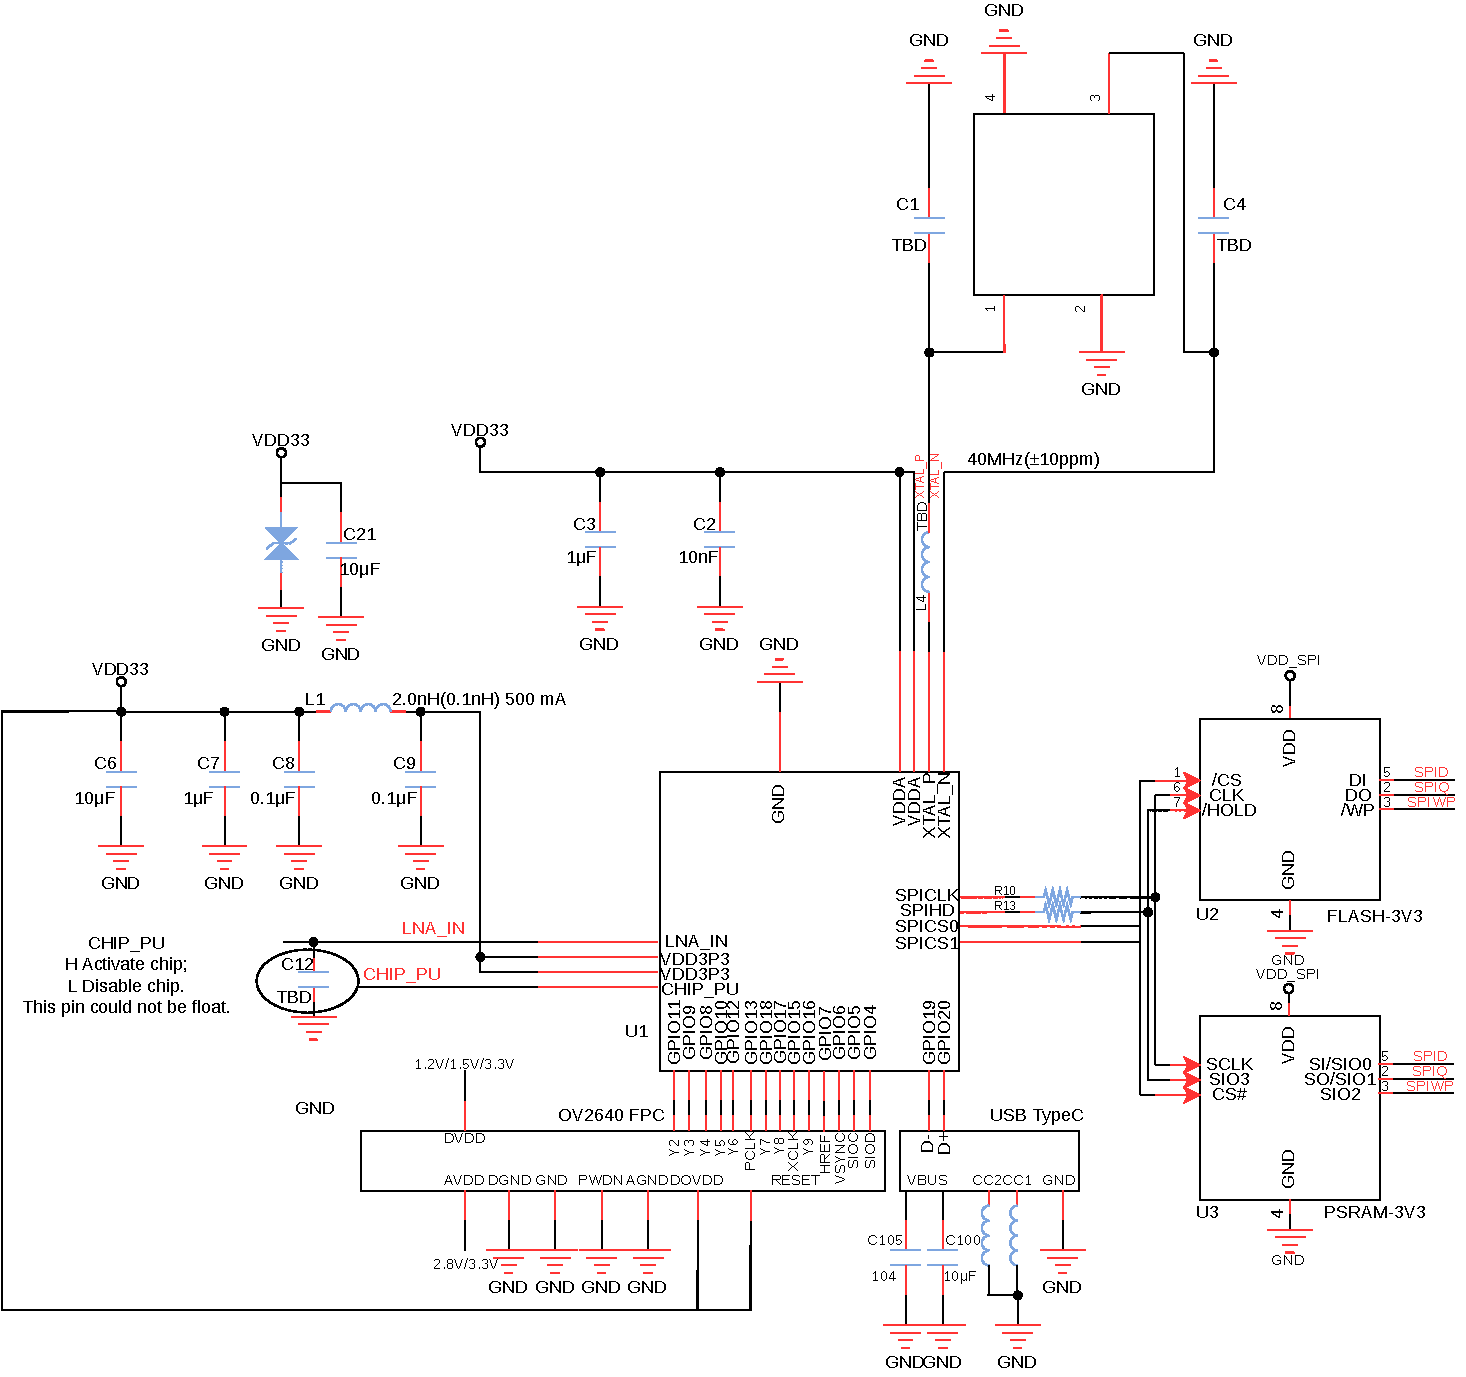
\includegraphics[width=1\textwidth]{./figures/原理图.pdf}
    \caption{原理图}
    \label{fig:原理图}
\end{figure}

\subsection{MCU 介绍}

ESP32-S3 本质上是一颗高集成度的 SoC，因为其系统目标就是处理器，所以也可以视为一颗 MCU\cite{yufanwei_mcu_soc}。我们只介绍该 MCU 中本项目涉及到的功能。

\subsubsection{系统}

\textbf{CPU}

ESP32-S3 采用 Xtensa® LX7 32 位双核处理器，具有如下特性：

\begin{itemize}
    \item 典型五级流水线架构，时钟频率达240MHz。
    \item 采用 Xtensa 指令集，支持半/全定制化指令集扩展。
    \item 支持 32 位乘法器、32 位除法器，适合分布式计算。
    \item 支持六级 32 个中断。
\end{itemize}

\textbf{指令扩展}

针对 AI 边缘和数字信号处理算法的运算效率，ESP32-S3新增了扩展指令和处理器功能。在原有 64 个物理通用寄存器的基础上新增 128 位宽通用寄存器，并提供 128 位宽的向量数据操作，合并数据处理指令与加载/存储运算指令。针对 128 位宽向量数据的潜在问题，底层实现了非对齐存取和取饱和操作。

\textbf{内部存储器}

ESP32-S3 的内部存储器即集成于芯片晶圆上或封装内部的存储器，包括 ROM、SRAM、eFuse 和 flash，各个存储元件具有不同特性：

\begin{enumerate}
    \item 384KB ROM：用于程序启动和内核功能调用。
    \item 512KB 片上SRAM：用于数据和指令存储。
    \item 8KB SRAM RTC 快速存储器：为处理器直接访问。
    \item 8KB SRAM RTC 慢速存储器：为处理器直接访问。
    \item 4096 位 eFuse 存储器。
    \item Flash、PSRAM：通过高频 SPI 总线外挂，后者是本项目用于图像缓冲区的重要组件。
\end{enumerate}

\subsubsection{外设}

\textbf{UART 控制器}

ESP32-S3 有三个UART控制器，支持异步通信和 IrDA，通信速率可达到 5Mbps。

\textbf{I2C 接口}

ESP32-S3 有两个 I2C 总线接口，可以用作 I2C 主机或从机模式。

\textbf{LCD 与 Camera 控制器}

LCD 模块用于发送并行视频数据信号，其总线 8 位 ~ 16 位并行 RGB、I8080、MOTO6800 接口，支持 RGB565、YUV422、YUV420、YUV411 之间的互相转换。

Camera 模块用于接收并行视频数据信号，其总线支持 8 位 ~ 16 位 DVP 图像传感器接口，支持 RGB565、YUV422、YUV420、YUV411 之间的互相转换。

在本项目中，OV2640 每一个像素时钟 (PCLK) 在 D0 ~ D7 上并行输出一个字节的数据，ESP32-S3 内部的 Camera 模块通过 DVP 控制器以硬件直接存取 (DMA) 的方式，将这些像素数据高速搬运到 PSRAM 内存中。此外 OV2640 输出的原始格式通常是 RGB565。而本项目采用的 MNIST 神经网络模型需要的是 $28\times28$ 单通道灰度图。Camera 模块可以在像素进入内存时直接进行色彩空间转换，从而降低 CPU 逐像素计算的软件开销。


\textbf{USB 2.0 OTG 全速接口}

ESP32-S3 带有一个集成了收发器的全速 USBOTG 外设，符合 USB2.0 规范。

我们会在讲解 Type-C 接口的时候再详细叙述。

\subsection{OV2640 摄像头}

本外设是在购买 ESP32-S3 开发板时附带的摄像头模块，其出厂即通过 FPC 柔性电路软板被翻盖锁扣锁定，撕掉镜头底座背面的双面胶纸后，即可将镜头按压粘在开发板的 PCB 板面上。此时还需要撕掉镜头镜头盖正面的微型透明防尘保护膜。

\textbf{参数}

OV2640 采用 1/4 英寸 CMOS 图像传感器，最高支持 200 万像素、每秒 15~60 帧图像采集。在本项目中，我们将其降采样为 $28\times28$ 以适应 MNIST 软件特征。借助片上 ISP，OV2640 可以通过自身 ISP Engine 在硬件层直接完成自动曝光、自动增益、自动白平衡和 JPEG 格式压缩，极大地减轻了 ESP32-S3 的计算负担。

\textbf{接口}

如原理图所示：并行数据线 $Y2\sim Y9$ 即 DVP 8 位数据总线 ($D0\sim D7$)，连接 ESP32-S3 的 GPIO11, 9, 8, 10, 12, 18, 17, 16；$PCLK$ (Pixel Clock) 连接像素时钟线 (GPIO13)。每当 $PCLK$ 时钟脉冲跳变一次，$D0\sim D7$ 的 8 根引脚上就会同时输出 1 个字节的像素数据。这里的图像是 RGB565 格式，当 $PCLK$ 敲击两次，$D0\sim D7$ 就会吐出 2 个字节，ESP32-S3 的 DMA 控制器就会自动把这 2 个字节组合成一个完整的像素点写入 PSRAM 内存。上述分析说明了本项目的采样频率和图像特点。

OV2640 上的 $VSYNC$ 连接 GPIO6，$HREF$ 连接 GPIO7。当摄像头准备传输新的一帧画面时，$VSYNC$ 将会拉低/拉高该引脚脉冲。当摄像头准备传输画面中的新一行像素时，将会激活$HREF$。这个原理和计算机系统综合设计中的 VGA 显示器显示原理是类似的。ESP32-S3 的 Camera 控制器依靠这两个硬件信号，把一连串连续流动的字节流，精准还原为内存中结构化的二维图像矩阵。

主时钟 $XCLK$ 连接 GPIO15。OV2640 芯片内部没有晶振，其内部时钟须依赖 ESP32-S3 驱动一个 $10MHz\sim 24MHz$ 的方波信号。ESP32-S3 先输出 $XCLK$ 心跳激活 OV2640，OV2640 才能根据这个内部倍频，进而产生 $PCLK$ 和像素数据提供给主控。

\section{设计思路}

本项目旨在探索受限资源单片机在机器视觉与人工智能领域的应用。在硬件平台选择上，80C51 较难胜任算力要求和内存要求高的数字图像识别任务。

ESP32-S3 具备 AI 加速指令集且具有可选 PSRAM 处理图像缓冲问题。

在环境配置阶段，选用了 Arduino IDE，平台信息会在软件部分叙述。克服工具链路径依赖问题后，我们成功构建了基于 C++ 的底层硬件驱动环境，为后续的软硬件协同开发奠定了基础。

\subsection{方案雏形}

Arduino IDE 提供了对 esp32 by espressif 下载源的支持。项目初期，通过部署 esp32 库提供的 CameraWebServer 示例，验证了 OV2640 摄像头的数据采集能力。单片机作为图像采集节点，可以将视频流通过 Wi-Fi 传输至局域网内的 PC 端。具体来说，如果示例占用了 X 端口，可以通过 \texttt{http://localhost:X/picture} 直接获取图像。尝试调用经典的 MNIST 神经网络模型进行阿拉伯数字的识别，我成功跑通了数字图像识别。

\begin{figure}[H]
    \centering
    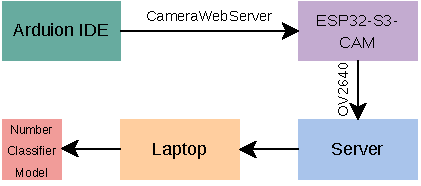
\includegraphics[width=1\textwidth]{./figures/方案雏形.pdf}
    \caption{方案雏形}
    \label{fig:方案雏形}
\end{figure}

这种传统的云/端分离架构存在缺陷：

\begin{itemize}
    \item 高度依赖 Wi-Fi 网络稳定性。
    \item 存在明显的网络传输延迟。
\end{itemize}

\subsection{初版方案}

注意到 MNIST 模型参数量极低，因此 AI 推理过程可以从 PC 端下放至 MCU 侧，实现真正的边缘计算。

具体来说，摄像头输出灰度图像，直接存入 ESP32-S3 的 PSRAM 帧缓冲区。设计裁剪逻辑提取 ROI (Region of Interest) ，从而下采样至 28x28 的特征张量。引入二值化反转算法，将现实中的白纸黑字动态转换为模型所需的黑底白字特征。最后将预处理后的张量送入通过 Edge Impulse 打包的片上 ONNX 视觉模型，提取 Logit 最高分映射为实际数字。本质上是利用 ESP32-S3 的双核 240MHz 算力与片上内存，直接在本地运行量化后的神经网络。

\begin{figure}[H]
    \centering
    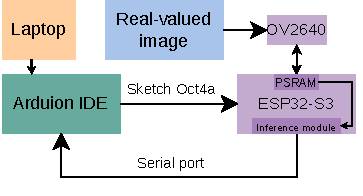
\includegraphics[width=1\textwidth]{./figures/初版方案.pdf}
    \caption{初版方案}
    \label{fig:初版方案}
\end{figure}

该方案成功实现了脱机的本地视觉识别，推理耗时控制在数百毫秒级，证明了 MCU 运行 AI 模型的完全可行性。作为初版方案，在实际测试中发现，传统的图像分类模型对数字在画面中的位置极其敏感，必须严格对准画面中心才能准确识别，鲁棒性仍有提升空间。

\subsection{终版方案}

为了解决初版方案影响图像截取的物理限制，终版方案将计算机视觉任务从\textbf{图像分类}升级为\textbf{目标检测}。即引入专为微控制器设计的 FOMO 目标检测架构，摒弃了锚框机制，转而预测画面中的目标中心点。以实现摄像头在完整的视野范围内，同时检测并框出图像中的人脸与佩戴口罩信息，并输出是否佩戴口罩。这使得整个系统可以进阶为具备工业分拣、智能计数潜力的完整边缘视觉设备。

\begin{figure}[H]
    \centering
    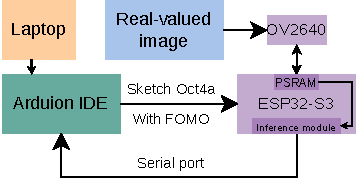
\includegraphics[width=1\textwidth]{./figures/终版方案.pdf}
    \caption{终版方案}
    \label{fig:终版方案}
\end{figure}

\section{设计功能点}

\subsection{方案雏形}

\begin{enumerate}
    \item 图像实时推流：ESP32-S3-CAM 通过 Wi-Fi HTTP 协议将 OV2640 捕获的视频流推送到 PC 端。需要注意，OV2640 本身没有固定的端到端传输延迟：若帧率为 15 FPS 或 30 FPS，仅等待下一帧就分别约需 67 ms 或 33 ms；实际延迟还包括曝光与读出、JPEG 编码、ESP32 缓冲及 Wi-Fi/HTTP 传输和 PC 端显示。因而总延迟取决于分辨率、帧率、缓冲策略和网络状况。通常能维持每秒15帧。
    \item 上位机辅助识别：PC 端接收视频流并调用 MNIST 模型进行阿拉伯数字分类与展示。由于不依赖单片机，这个过程特别快。
\end{enumerate}

\subsection{初版方案}

\begin{enumerate}
    \item 脱机本地推理：不依赖 Wi-Fi 传输，由 ESP32-S3 片上直接运行 MNIST 图像分类模型。
    \item 硬件预处理：对采集到的图像进行中心 160x160 ROI 裁剪、28x28 缩放以及二值化黑白反转。
    \item 串口数据反馈：实时通过 UART 串口输出识别出的数字类别、置信度 Score 和片上推理耗时。
\end{enumerate}

上述初版方案识别一次结果通常耗时约 1400ms。

\subsection{终版方案}

\begin{enumerate}
    \item 智能识别：取消中心裁剪限制，在完整视野范围内自动寻找人脸。
    \item 多目标检测与定位：基于 FOMO 极轻量目标检测架构，支持识别并定位画面中人脸与是否佩戴口罩信息。
    \item 串口数据反馈：串口输出推理结果与置信度外，实时吐出检测每个目标的耗时。
\end{enumerate}

由于改进了模型导出策略，不同于初版方案全量识别，终版方案识别一次结果通常耗时约 140ms。

\section{软件设计}

本项目的软件侧涉及四个平台，如下呈现了它们各自的职责：

\begin{table}[H]
\centering
\caption{软件侧平台职责}
\begin{tabular}{L{4cm} L{9.5cm}}
\toprule
\textbf{平台} & \textbf{职责} \\
\midrule
\texttt{VisualStudioCode} & 模型获取、数据集获取、模型训练 \\
\texttt{Arduino IDE} & 确定硬件行为、导入位流 \\
\texttt{Edge Impulse}  & 模型训练、模型打包 \\
\texttt{Roboflow Universe}   & 获取数据集 \\
\bottomrule
\end{tabular}
\end{table}

后续会介绍各个方案的软件设计，会区分各个方案使用平台的不同。

\subsection{方案雏形}

首先需要说明该方案在 Arduino IDE 平台上的代码非本人所做，而是来自于 esp32 开发板环境示例 \texttt{CameraWebServer}。我在此基础上做了少量修改，只展示涉及修改的部分。

\textbf{根据板子型号规定针脚使用}

\begin{lstlisting}[language=C++,caption={定义针脚}]
/// board_config.h
#ifndef BOARD_CONFIG_H
#define BOARD_CONFIG_H

#define CAMERA_MODEL_ESP32S3_EYE  // Has PSRAM
#include "camera_pins.h"

#endif  // BOARD_CONFIG_H

/// camera_pins.h
#if defined(CAMERA_MODEL_WROVER_KIT)
// ...

#elif defined(CAMERA_MODEL_ESP32S3_EYE)
#define PWDN_GPIO_NUM  -1
#define RESET_GPIO_NUM -1
#define XCLK_GPIO_NUM  15
#define SIOD_GPIO_NUM  4
#define SIOC_GPIO_NUM  5

#define Y2_GPIO_NUM 11
#define Y3_GPIO_NUM 9
#define Y4_GPIO_NUM 8
#define Y5_GPIO_NUM 10
#define Y6_GPIO_NUM 12
#define Y7_GPIO_NUM 18
#define Y8_GPIO_NUM 17
#define Y9_GPIO_NUM 16

#define VSYNC_GPIO_NUM 6
#define HREF_GPIO_NUM  7
#define PCLK_GPIO_NUM  13
\end{lstlisting}

上述代码根据开发板原理图规定了摄像头的各个针脚与 ESP32-S3 的 GPIO 之间的映射关系。后续方案会以不同方式遵循这些针脚映射。

根据 \texttt{CameraWebServer} 的设计，硬件会返回 \texttt{ESP32\_IP}，在 PC 端访问 \texttt{http://ESP32\_IP/picture} 即可获取摄像头的 JPEG 图像。在本地实现 MNIST 模型推理的过程中，只需要将 JPEG 图像送入即可：

\begin{lstlisting}[language=Python,caption={本地模型推理}]
import cv2
import numpy as np
import urllib.request
from torchvision import transforms

onnx_url = "https://github.com/onnx/models/raw/main/validated/vision/classification/mnist/model/mnist-12.onnx"
model_path = "mnist-12.onnx"

# 下载 ONNX 模型
urllib.request.urlretrieve(onnx_url, model_path)

# 加载 ONNX 模型
net = cv2.dnn.readNetFromONNX(model_path)

# 读取图像并输入模型推理
def predict_digit(img_28x28):
    # 归一化并转为 blob 格式 [1, 1, 28, 28]
    blob = cv2.dnn.blobFromImage(img_28x28, 1.0 / 255.0, (28, 28), (0, 0, 0), swapRB=False, crop=False)
    net.setInput(blob)
    outputs = net.forward()
    prediction = np.argmax(outputs)
    confidence = np.max(cv2.softmax(outputs)) if hasattr(cv2, 'softmax') else np.exp(outputs[0][prediction]) / np.sum(np.exp(outputs[0]))
    return prediction, confidence

if __name__ == "__main__":
    # 这是上次实验默认的 ESP32-S3-CAM IP 地址
    ESP32_IP = "192.168.2.17"
    URL = f"http://{ESP32_IP}/capture"

    transform = transforms.Compose([
        transforms.ToTensor(),
        transforms.Normalize((0.1307,), (0.3081,))
    ])

    while True:
        try:
            # 抓取一帧 JPEG 图像
            img_resp = urllib.request.urlopen(URL, timeout=5)
            img_np = np.array(bytearray(img_resp.read()), dtype=np.uint8)
            frame = cv2.imdecode(img_np, -1)

            if frame is None:
                continue

            gray = cv2.cvtColor(frame, cv2.COLOR_BGR2GRAY)
            blurred = cv2.GaussianBlur(gray, (5, 5), 0)
            _, thresh = cv2.threshold(blurred, 0, 255, cv2.THRESH_BINARY_INV + cv2.THRESH_OTSU)

            resized = cv2.resize(thresh, (28, 28), interpolation=cv2.INTER_AREA)

            prediction, confidence = predict_digit(resized)

            display_frame = frame.copy()
            text = f"Digit: {prediction} ({confidence*100:.1f}%)"
            cv2.putText(display_frame, text, (20, 40), cv2.FONT_HERSHEY_SIMPLEX, 1, (0, 255, 0), 2)

            cv2.imshow("ESP32-S3 Digital Recognition", display_frame)
            cv2.imshow("Model Input (28x28)", cv2.resize(thresh, (280, 280)))

            if cv2.waitKey(1) & 0xFF == ord('q'):
                break

        except Exception as e:
            print(f"图像获取或推理异常: {e}")
            break

    cv2.destroyAllWindows()
\end{lstlisting}

\subsection{初版方案}

首先需要完成把推理模型打包的过程，此后才能嵌入 ESP-S3。先说明模型来源。可以使用上一个方案直接获取的模型文件：

\begin{lstlisting}[language=Python,caption={下载 MNIST ONNX 模型}]
import urllib.request

onnx_url = "https://github.com/onnx/models/raw/main/validated/vision/classification/mnist/model/mnist-12.onnx"
model_path = "mnist-12.onnx"
urllib.request.urlretrieve(onnx_url, model_path)
\end{lstlisting}

也可以自己搭建卷积神经网络训练一个模型文件。经过实际测试，这两个模型文件的效果没有太大区别：

\begin{lstlisting}[language=Python,caption={训练 MNIST 模型}]
import torch
import torch.nn as nn
import torch.optim as optim
from torchvision import datasets, transforms
from torch.utils.data import DataLoader

# MNIST CNN
class MNISTModel(nn.Module):
    def __init__(self):
        super(MNISTModel, self).__init__()
        # 第一层卷积：输入 1 通道，输出 16 通道，卷积核 5x5
        self.conv1 = nn.Conv2d(1, 16, kernel_size=5, stride=1, padding=2)
        self.relu1 = nn.ReLU()
        self.pool1 = nn.MaxPool2d(kernel_size=2, stride=2) # 输出 14x14
        
        # 第二层卷积：输入 16 通道，输出 32 通道，卷积核 5x5
        self.conv2 = nn.Conv2d(16, 32, kernel_size=5, stride=1, padding=2)
        self.relu2 = nn.ReLU()
        self.pool2 = nn.MaxPool2d(kernel_size=2, stride=2) # 输出 7x7
        
        # 全连接分类层：32 * 7 * 7 = 1568 -> 10 个分类
        self.fc1 = nn.Linear(32 * 7 * 7, 128)
        self.relu3 = nn.ReLU()
        self.fc2 = nn.Linear(128, 10)

    def forward(self, x):
        x = self.pool1(self.relu1(self.conv1(x)))
        x = self.pool2(self.relu2(self.conv2(x)))
        x = x.view(x.size(0), -1)
        x = self.relu3(self.fc1(x))
        x = self.fc2(x)
        return x

# MNIST 数据集
transform = transforms.Compose([
    transforms.ToTensor(),
    transforms.Normalize((0.1307,), (0.3081,))
])

train_dataset = datasets.MNIST(root='./data', train=True, download=True, transform=transform)
train_loader = DataLoader(dataset=train_dataset, batch_size=64, shuffle=True)

device = torch.device("cuda" if torch.cuda.is_available() else "cpu")
model = MNISTModel().to(device)
criterion = nn.CrossEntropyLoss()
optimizer = optim.Adam(model.parameters(), lr=0.001)

model.train()
for epoch in range(3):
    running_loss = 0.0
    for i, (images, labels) in enumerate(train_loader):
        images, labels = images.to(device), labels.to(device)
        
        optimizer.zero_grad()
        outputs = model(images)
        loss = criterion(outputs, labels)
        loss.backward()
        optimizer.step()
        
        running_loss += loss.item()
    print(f"Epoch [{epoch+1}/3], Loss: {running_loss / len(train_loader):.4f}")

model.eval()
dummy_input = torch.randn(1, 1, 28, 28, device=device)

onnx_filename = "mnist-12.onnx"
torch.onnx.export(
    model,
    dummy_input,
    onnx_filename,
    export_params=True,
    opset_version=12,
    do_constant_folding=True,
    input_names=['Input3'],
    output_names=['Plus214_Output_0'],
    dynamic_axes={
        'Input3': {0: 'batch_size'},
        'Plus214_Output_0': {0: 'batch_size'}
    }
)

print(f"导出 ONNX 模型: {onnx_filename}")
\end{lstlisting}

接着通过 Edge Impulse 把模型打包成Arduino IDE 可用的位流文件。具体来说：

\begin{enumerate}
    \item 在 Edge Impulse 平台上传 \texttt{mnist-12.onnx} 模型文件。
    \item 配置模型参数，包括输入输出维度、量化选项等。
    \item 以 Arduino library 格式导出模型，生成位流文件。
\end{enumerate}

即可获得库文件，在 Arduino IDE 中导入该库文件后，即可编写嵌入模型到 ESP32-S3 上运行的代码：

\begin{lstlisting}[language=C++,caption={嵌入模型到 ESP32-S3}]
#include <Test_inferencing.h>

#include "esp_camera.h"
#include "Arduino.h"

// 上一步导出库文件的头文件
#include <Test_inferencing.h>

// 参见方案雏形
#define PWDN_GPIO_NUM     -1
#define RESET_GPIO_NUM    -1
#define XCLK_GPIO_NUM     15
#define SIOD_GPIO_NUM      4
#define SIOC_GPIO_NUM      5

#define Y9_GPIO_NUM       16
#define Y8_GPIO_NUM       17
#define Y7_GPIO_NUM       18
#define Y6_GPIO_NUM       12
#define Y5_GPIO_NUM       10
#define Y4_GPIO_NUM        8
#define Y3_GPIO_NUM        9
#define Y2_GPIO_NUM       11

#define VSYNC_GPIO_NUM     6
#define HREF_GPIO_NUM      7
#define PCLK_GPIO_NUM     13

#define RAW_BUF_WIDTH  320
#define RAW_BUF_HEIGHT 240

static float features[EI_CLASSIFIER_INPUT_WIDTH * EI_CLASSIFIER_INPUT_HEIGHT];

static int raw_feature_get_data(size_t offset, size_t length, float *out_ptr) {
    memcpy(out_ptr, features + offset, length * sizeof(float));
    return 0;
}

void setup() {
    Serial.begin(115200);
    delay(2000); 
    while (!Serial && millis() < 5000);

    camera_config_t config;
    config.ledc_channel = LEDC_CHANNEL_0;
    config.ledc_timer = LEDC_TIMER_0;
    config.pin_d0 = Y2_GPIO_NUM;
    config.pin_d1 = Y3_GPIO_NUM;
    config.pin_d2 = Y4_GPIO_NUM;
    config.pin_d3 = Y5_GPIO_NUM;
    config.pin_d4 = Y6_GPIO_NUM;
    config.pin_d5 = Y7_GPIO_NUM;
    config.pin_d6 = Y8_GPIO_NUM;
    config.pin_d7 = Y9_GPIO_NUM;
    config.pin_xclk = XCLK_GPIO_NUM;
    config.pin_pclk = PCLK_GPIO_NUM;
    config.pin_vsync = VSYNC_GPIO_NUM;
    config.pin_href = HREF_GPIO_NUM;
    config.pin_sccb_sda = SIOD_GPIO_NUM;
    config.pin_sccb_scl = SIOC_GPIO_NUM;
    config.pin_pwdn = PWDN_GPIO_NUM;
    config.pin_reset = RESET_GPIO_NUM;
    config.xclk_freq_hz = 10000000;
    config.pixel_format = PIXFORMAT_GRAYSCALE; 
    config.frame_size = FRAMESIZE_QVGA;
    config.jpeg_quality = 12;
    config.fb_count = 1;
    config.fb_location = CAMERA_FB_IN_PSRAM;

    esp_err_t err = esp_camera_init(&config);
    if (err != ESP_OK) {
        Serial.printf("[Error] Camera initialized failed: 0x%x\n", err);
        while (1);
    }
    sensor_t * s = esp_camera_sensor_get();
    
    s->set_vflip(s, 1);
    
    Serial.println("[Info] Model loaded\n");
}

void loop() {
    camera_fb_t *fb = esp_camera_fb_get();
    if (!fb) {
        Serial.println("[Warn] Picture captured failed");
        delay(500);
        return;
    }

    int crop_size = 160;
    int start_x = (RAW_BUF_WIDTH - crop_size) / 2;
    int start_y = (RAW_BUF_HEIGHT - crop_size) / 2;
    float scale = (float)crop_size / EI_CLASSIFIER_INPUT_WIDTH;

    for (int y = 0; y < EI_CLASSIFIER_INPUT_HEIGHT; y++) {
        for (int x = 0; x < EI_CLASSIFIER_INPUT_WIDTH; x++) {
            int src_x = start_x + (int)(x * scale);
            int src_y = start_y + (int)(y * scale);
            
            uint8_t raw_pixel = fb->buf[src_y * RAW_BUF_WIDTH + src_x];

            uint8_t val = (raw_pixel < 120) ? 255 : 0; 

            uint32_t rgb_pixel = (val << 16) | (val << 8) | val;
            
            features[y * EI_CLASSIFIER_INPUT_WIDTH + x] = (float)rgb_pixel;
        }
    }

    esp_camera_fb_return(fb);

    signal_t signal;
    signal.total_length = EI_CLASSIFIER_INPUT_WIDTH * EI_CLASSIFIER_INPUT_HEIGHT;
    signal.get_data = &raw_feature_get_data;

    Serial.println("\n--- 28x28 input preview ---");
    for (int y = 0; y < EI_CLASSIFIER_INPUT_HEIGHT; y++) {
        for (int x = 0; x < EI_CLASSIFIER_INPUT_WIDTH; x++) {
            float p = features[y * EI_CLASSIFIER_INPUT_WIDTH + x];
            Serial.print(p > 0.0f ? "#" : "."); 
        }
        Serial.println();
    }

    ei_impulse_result_t result = { 0 };
    EI_IMPULSE_ERROR res = run_classifier(&signal, &result, false);

    if (res != EI_IMPULSE_OK) {
        Serial.printf("[Error] Local reasoning failed (%d)\n", res);
        delay(1000);
        return;
    }

    int max_idx = -1;
    float max_val = -9999.0f;

    for (size_t i = 0; i < EI_CLASSIFIER_LABEL_COUNT; i++) {
        if (result.classification[i].value > max_val) {
            max_val = result.classification[i].value;
            max_idx = i;
        }
    }

    if (max_idx >= 0) {
        int recognized_digit = max_idx; 
        
        Serial.printf("-> Recognized result: %d | Score: %.2f | time usage: %d ms\n",
                      recognized_digit,
                      result.classification[max_idx].label,
                      max_val,
                      result.timing.classification);
    }

    delay(500); 
}
\end{lstlisting}

此时，ESP32-S3-CAM 就可以在本地完成图像采集、预处理和 MNIST 模型推理，并通过串口输出识别结果。

\subsection{终版方案}

本方案与初版方案的区别主要在于模型选用的区别，在此简单说明本方案使用的 FOMO 模型与初版方案使用的 MNIST 模型的不同。

\begin{table}[H]
\centering
\caption{模型比较}
\begin{tabular}{L{3cm} L{6cm} L{6cm}}
\toprule
\textbf{维度} & \textbf{MNIST} & \textbf{FOMO} \\
\midrule
\texttt{任务类型} & 图像分类 & 目标检测 \\
\texttt{图像预处理要求} & 极高，涉及灰度化及硬二值化 & 较低，使用原始灰度像素点数据 \\
\texttt{ESP32 运行效率}  & 较低，涉及很多模型外图像处理 & 较高，推理耗时固定 \\
\bottomrule
\end{tabular}
\end{table}

不同于初版方案，本方案模型的获取参考了开源项目 SSCMA\cite{sscmanual_mcu_soc}，只说明借助该项目获取模型文件的流程。

\begin{enumerate}
    \item 获取模型训练仓库 \href{https://github.com/Seeed-Studio/ModelAssistant}。
    \item 访问 \href{https://files.seeedstudio.com/sscma/datasets/coco_mask.zip} 获取 COCO Mask 数据集并解压缩到项目根目录。
    \item 执行
    \begin{lstlisting}[language=python,caption={训练 FOMO 模型}]
python tools/train.py \
    configs/fomo/fomo_mobnetv2_0.35_x8_coco.py \
    --cfg-options \
    data_root=coco_mask/mask/ \
    num_classes=2 \
    train_ann=train/_annotations.coco.json \
    val_ann=valid/_annotations.coco.json \
    train_data=train/ \
    val_data=valid/ \
    epochs=50 \
    height=192 \
    width=192
    \end{lstlisting}
    \item 将模型文件导入 Edge Impulse 平台，进行必要的配置和打包。
\end{enumerate}

由于模型功能不同，嵌入模型到 ESP32-S3 的代码也有差异，主要体现在图像预处理和结果处理部分：

\begin{lstlisting}[language=C++,caption={嵌入 FOMO 模型到 ESP32-S3}]
#include <Test_inferencing.h>

#include "esp_camera.h"
#include "Arduino.h"

#define PWDN_GPIO_NUM     -1
#define RESET_GPIO_NUM    -1
#define XCLK_GPIO_NUM     15
#define SIOD_GPIO_NUM      4
#define SIOC_GPIO_NUM      5

#define Y9_GPIO_NUM       16
#define Y8_GPIO_NUM       17
#define Y7_GPIO_NUM       18
#define Y6_GPIO_NUM       12
#define Y5_GPIO_NUM       10
#define Y4_GPIO_NUM        8
#define Y3_GPIO_NUM        9
#define Y2_GPIO_NUM       11

#define VSYNC_GPIO_NUM     6
#define HREF_GPIO_NUM      7
#define PCLK_GPIO_NUM     13

#define RAW_BUF_WIDTH  320
#define RAW_BUF_HEIGHT 240

static float features[EI_CLASSIFIER_INPUT_WIDTH * EI_CLASSIFIER_INPUT_HEIGHT];

static int raw_feature_get_data(size_t offset, size_t length, float *out_ptr) {
    memcpy(out_ptr, features + offset, length * sizeof(float));
    return 0;
}

void setup() {
    Serial.begin(115200);
    delay(2000); 
    while (!Serial && millis() < 5000);

    camera_config_t config;
    config.ledc_channel = LEDC_CHANNEL_0;
    config.ledc_timer = LEDC_TIMER_0;
    config.pin_d0 = Y2_GPIO_NUM;
    config.pin_d1 = Y3_GPIO_NUM;
    config.pin_d2 = Y4_GPIO_NUM;
    config.pin_d3 = Y5_GPIO_NUM;
    config.pin_d4 = Y6_GPIO_NUM;
    config.pin_d5 = Y7_GPIO_NUM;
    config.pin_d6 = Y8_GPIO_NUM;
    config.pin_d7 = Y9_GPIO_NUM;
    config.pin_xclk = XCLK_GPIO_NUM;
    config.pin_pclk = PCLK_GPIO_NUM;
    config.pin_vsync = VSYNC_GPIO_NUM;
    config.pin_href = HREF_GPIO_NUM;
    config.pin_sccb_sda = SIOD_GPIO_NUM;
    config.pin_sccb_scl = SIOC_GPIO_NUM;
    config.pin_pwdn = PWDN_GPIO_NUM;
    config.pin_reset = RESET_GPIO_NUM;
    config.xclk_freq_hz = 10000000;
    config.pixel_format = PIXFORMAT_GRAYSCALE; 
    config.frame_size = FRAMESIZE_QVGA;
    config.jpeg_quality = 12;
    config.fb_count = 1;
    config.fb_location = CAMERA_FB_IN_PSRAM;

    esp_err_t err = esp_camera_init(&config);
    if (err != ESP_OK) {
        Serial.printf("[Error] Camera initialized failed: 0x%x\n", err);
        while (1);
    }
    sensor_t * s = esp_camera_sensor_get();
    s->set_vflip(s, 1);
    
    Serial.println("[Info] FOMO Model and Camera initialized successfully\n");
}

void loop() {
    camera_fb_t *fb = esp_camera_fb_get();
    if (!fb) {
        Serial.println("[Warn] Picture captured failed");
        delay(500);
        return;
    }

    int crop_size = 160;
    int start_x = (RAW_BUF_WIDTH - crop_size) / 2;
    int start_y = (RAW_BUF_HEIGHT - crop_size) / 2;
    float scale = (float)crop_size / EI_CLASSIFIER_INPUT_WIDTH;

    for (int y = 0; y < EI_CLASSIFIER_INPUT_HEIGHT; y++) {
        for (int x = 0; x < EI_CLASSIFIER_INPUT_WIDTH; x++) {
            int src_x = start_x + (int)(x * scale);
            int src_y = start_y + (int)(y * scale);
            
            uint8_t raw_pixel = fb->buf[src_y * RAW_BUF_WIDTH + src_x];

            uint8_t val = raw_pixel;

            uint32_t rgb_pixel = (val << 16) | (val << 8) | val;
            features[y * EI_CLASSIFIER_INPUT_WIDTH + x] = (float)rgb_pixel;
        }
    }

    esp_camera_fb_return(fb);

    signal_t signal;
    signal.total_length = EI_CLASSIFIER_INPUT_WIDTH * EI_CLASSIFIER_INPUT_HEIGHT;
    signal.get_data = &raw_feature_get_data;

    ei_impulse_result_t result = { 0 };
    EI_IMPULSE_ERROR res = run_classifier(&signal, &result, false);

    if (res != EI_IMPULSE_OK) {
        Serial.printf("[Error] Local inference failed (%d)\n", res);
        delay(1000);
        return;
    }

    bool bb_found = false;
    Serial.printf("Inference timing: DSP %d ms, Classification %d ms\n",
                  result.timing.dsp, result.timing.classification);

#if EI_CLASSIFIER_OBJECT_DETECTION == 1
    for (size_t i = 0; i < EI_CLASSIFIER_OBJECT_DETECTION_COUNT; i++) {
        auto bb = result.bounding_boxes[i];
        
        if (bb.value < 0.5f) { 
            continue;
        }
        
        bb_found = true;
        Serial.printf("  -> Detected target: %s (Score: %.2f) | Center Box [ x: %u, y: %u, w: %u, h: %u ]\n",
                      bb.label,
                      bb.value,
                      bb.x,
                      bb.y,
                      bb.width,
                      bb.height);
    }
#endif

    if (!bb_found) {
        Serial.println("  -> No target detected.");
    }

    delay(200); 
}
\end{lstlisting}

此时，ESP32-S3-CAM 就可以在本地完成图像采集、预处理和 FOMO 模型推理，并通过串口输出识别结果。

\section{运行效果}

由于方案雏形不涉及边缘 AI 计算且大部分工作都是已有代码的增量工作，因此不再赘述。初版方案和终版方案的运行效果如下。

\subsection{初版方案}

\begin{figure}[H]
  \centering
  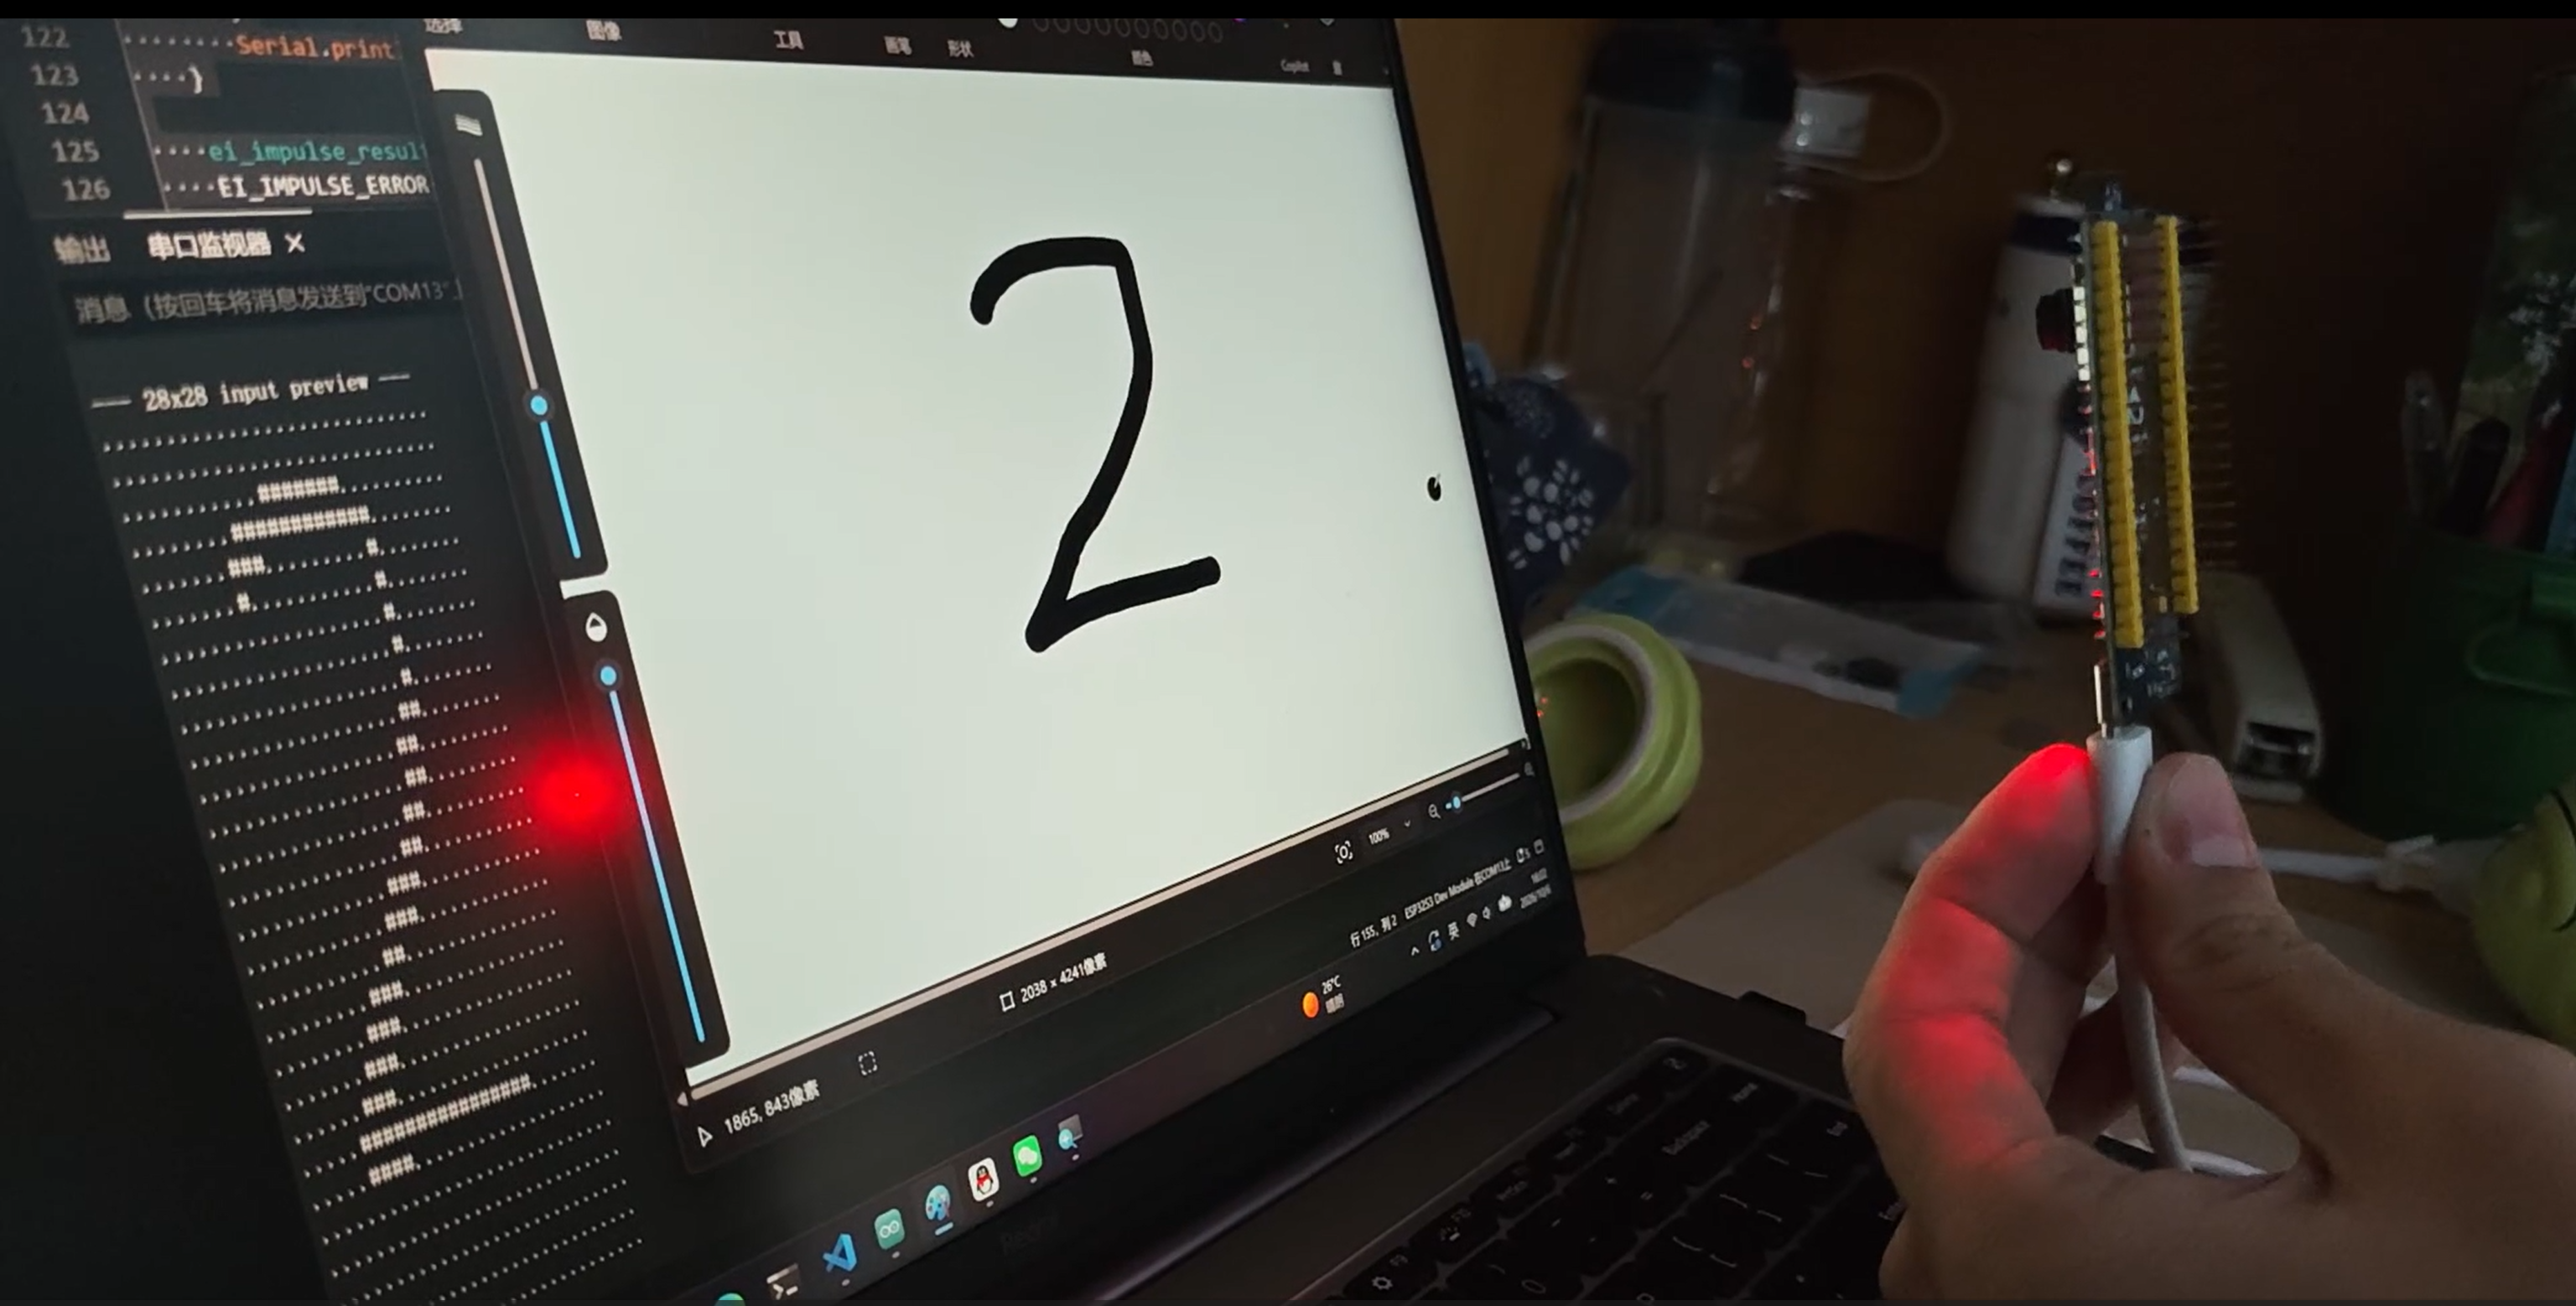
\includegraphics[width=0.5\linewidth]{figures/初版方案.png}\\[1em]
  \href{https://www.bilibili.com/video/BV1KCHf6eEz3}{点击此处查看演示视频} 
  \quad
  \qrcode[height=2cm]{https://www.bilibili.com/video/BV1KCHf6eEz3}
\end{figure}

\subsection{终版方案}

\begin{figure}[H]
  \centering
  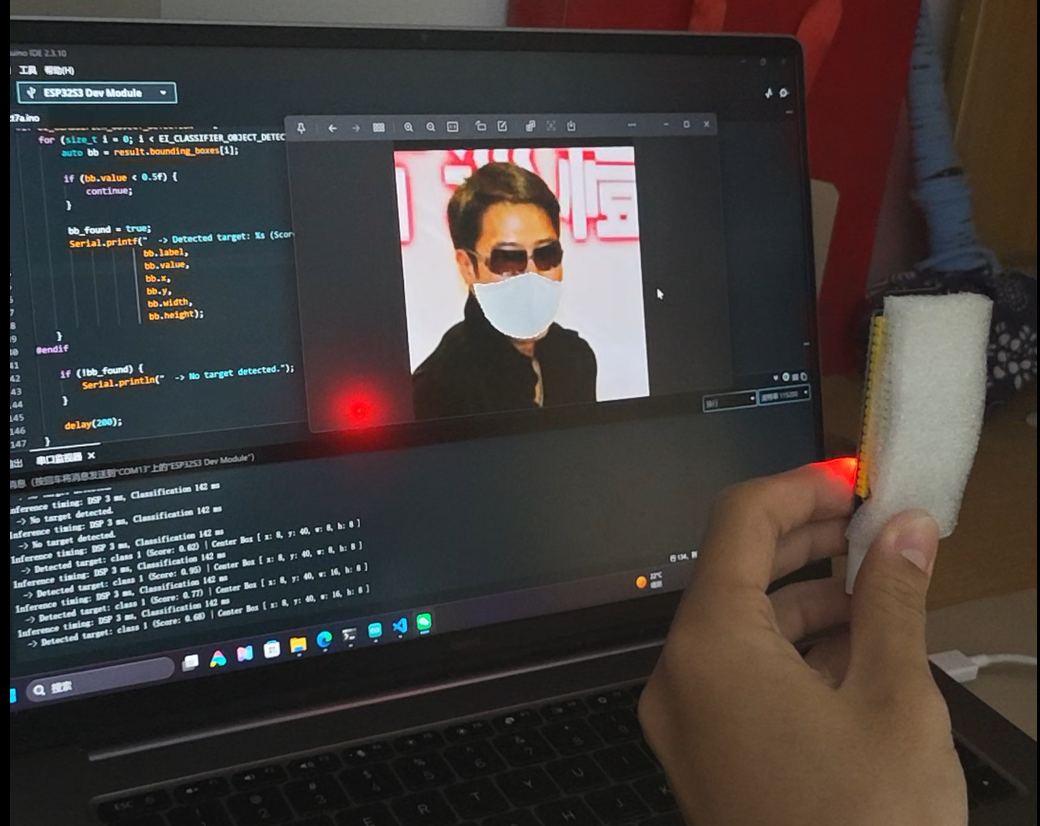
\includegraphics[width=0.5\linewidth]{figures/终版方案.png}\\[1em]
  \href{https://www.bilibili.com/video/BV1tepK69EHY}{点击此处查看演示视频} 
  \quad
  \qrcode[height=2cm]{https://www.bilibili.com/video/BV1tepK69EHY}
\end{figure}

\bibliographystyle{plain}
\bibliography{references}

\end{document}
